\mychapter{Additional Architectures/Graphs\label{app:B}}

\begin{figure}[h!]
\centering

\begin{subfigure}[t]{0.25\textwidth}
\centering
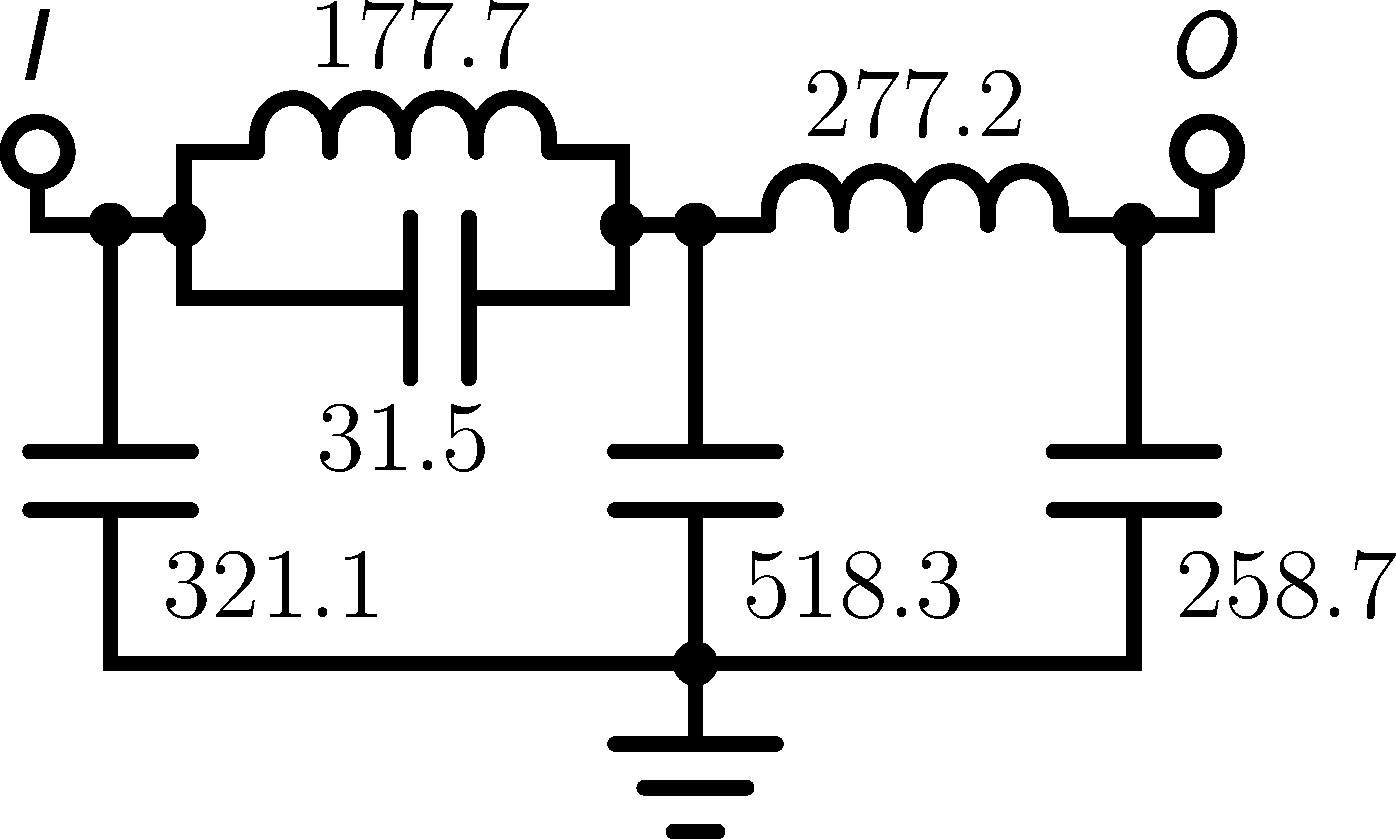
\includegraphics[scale = 0.14]{../ch6/figures/lpf3_circuit1}
\caption{}
\end{subfigure}%
\begin{subfigure}[t]{0.25\textwidth}
\centering
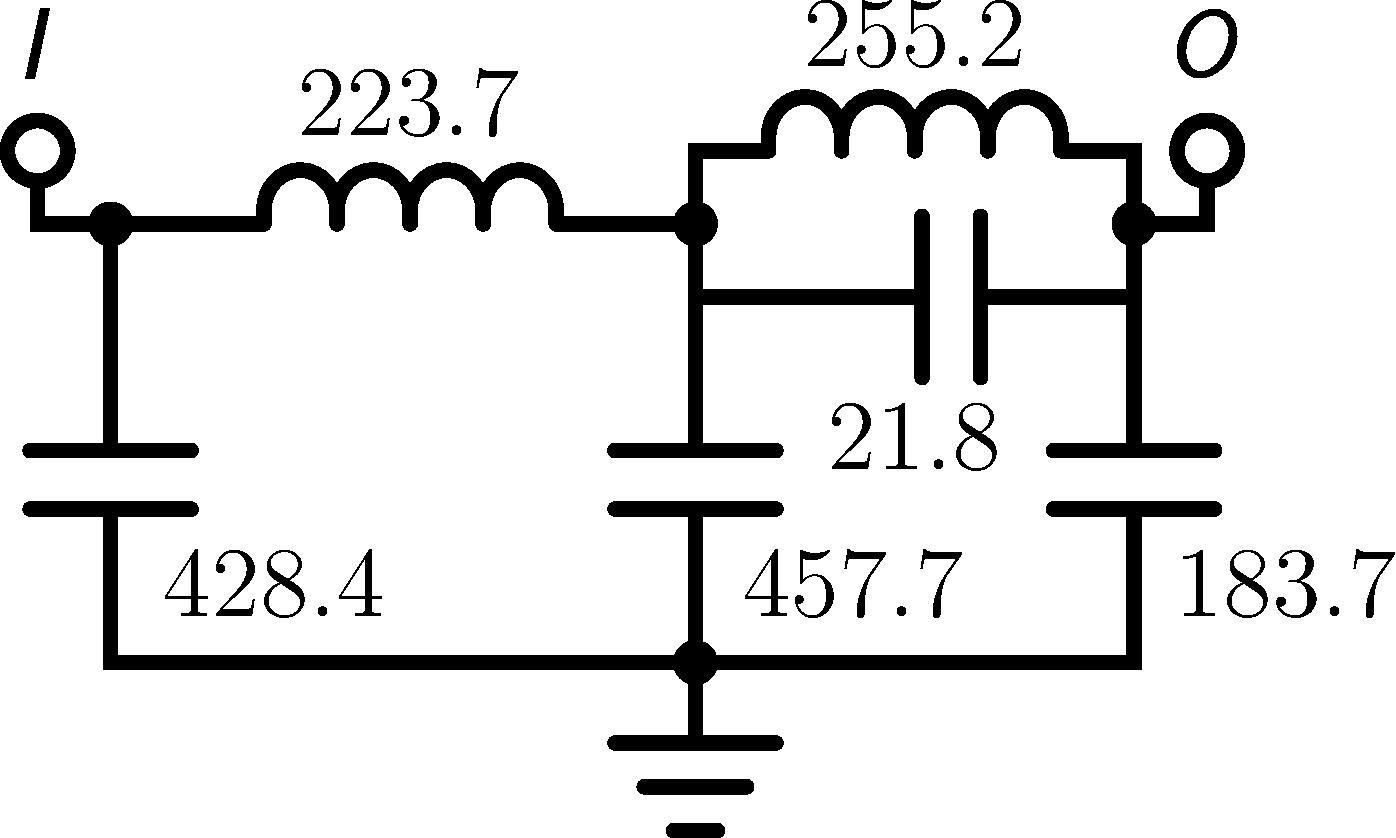
\includegraphics[scale = 0.14]{../app2/figures/(2)}
\caption{}
\end{subfigure}%

\begin{subfigure}[t]{0.25\textwidth}
\centering
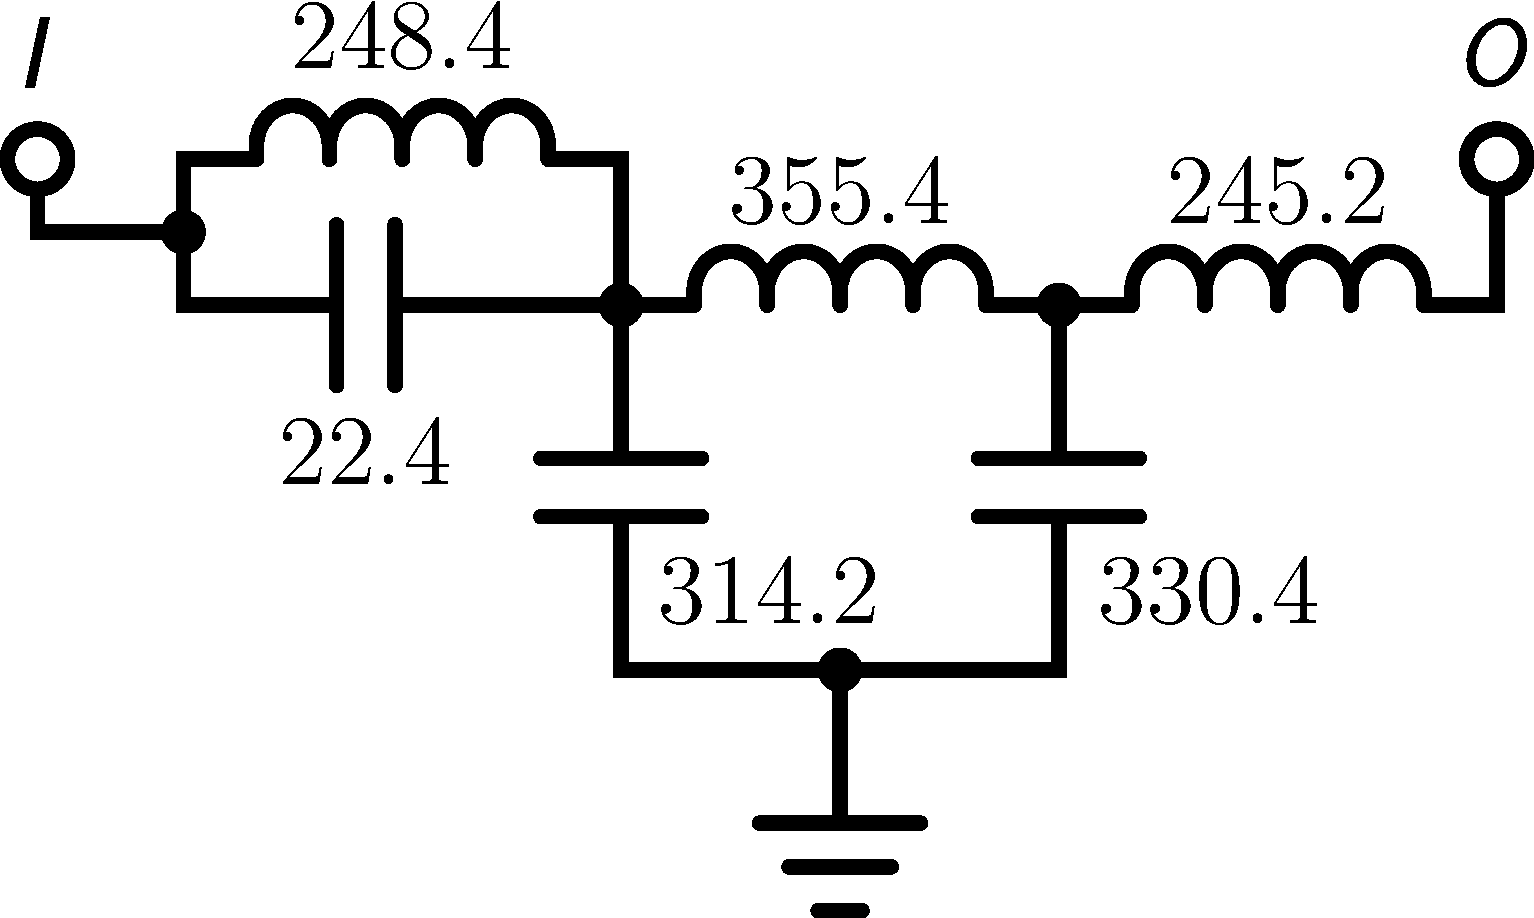
\includegraphics[scale = 0.14]{../app2/figures/(4)}
\caption{}
\end{subfigure}%
\begin{subfigure}[t]{0.25\textwidth}
\centering
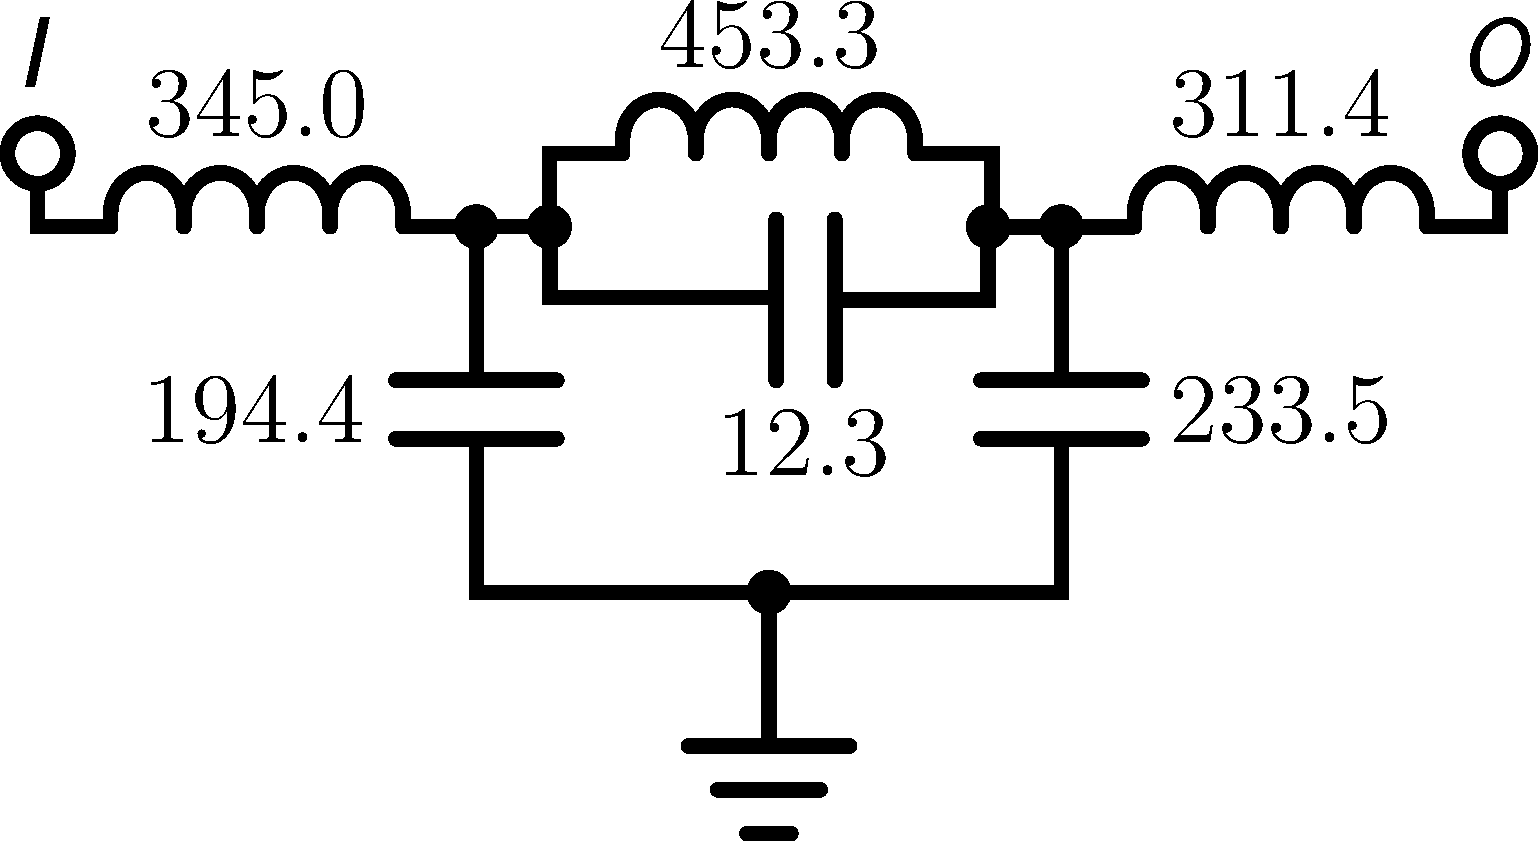
\includegraphics[scale = 0.14]{../ch6/figures/lpf3_circuit4}
\caption{}
\end{subfigure}%
\begin{subfigure}[t]{0.25\textwidth}
\centering
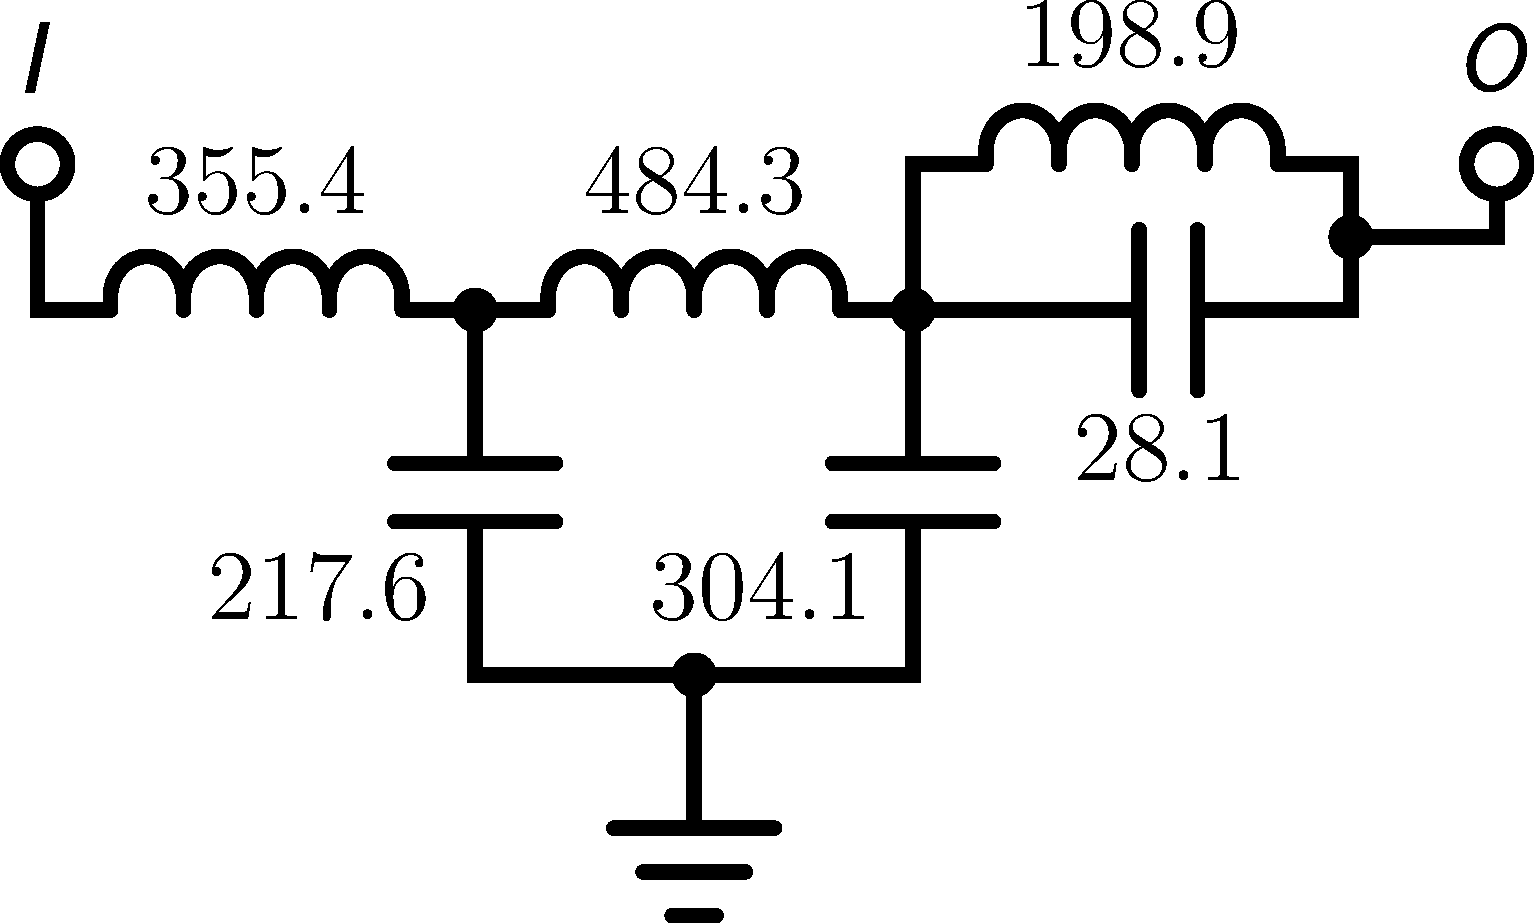
\includegraphics[scale = 0.14]{../ch6/figures/lpf3_circuit2}
\caption{}
\end{subfigure}%

\begin{subfigure}[t]{0.25\textwidth}
\centering
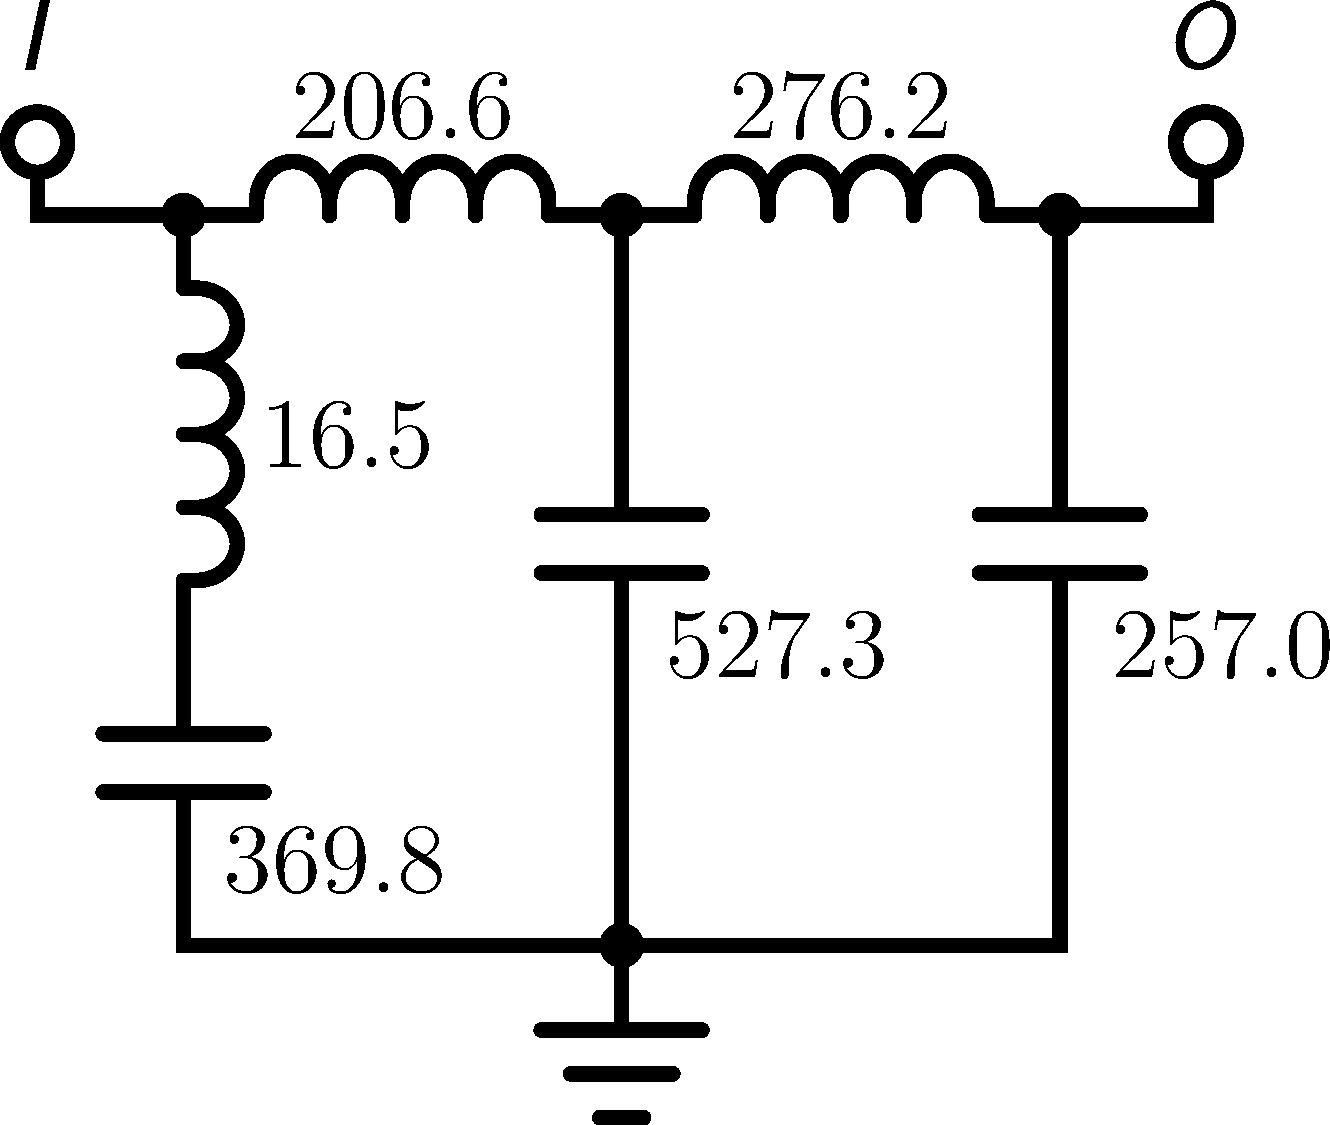
\includegraphics[scale = 0.14]{../app2/figures/(5)}
\caption{}
\end{subfigure}%
\begin{subfigure}[t]{0.25\textwidth}
\centering
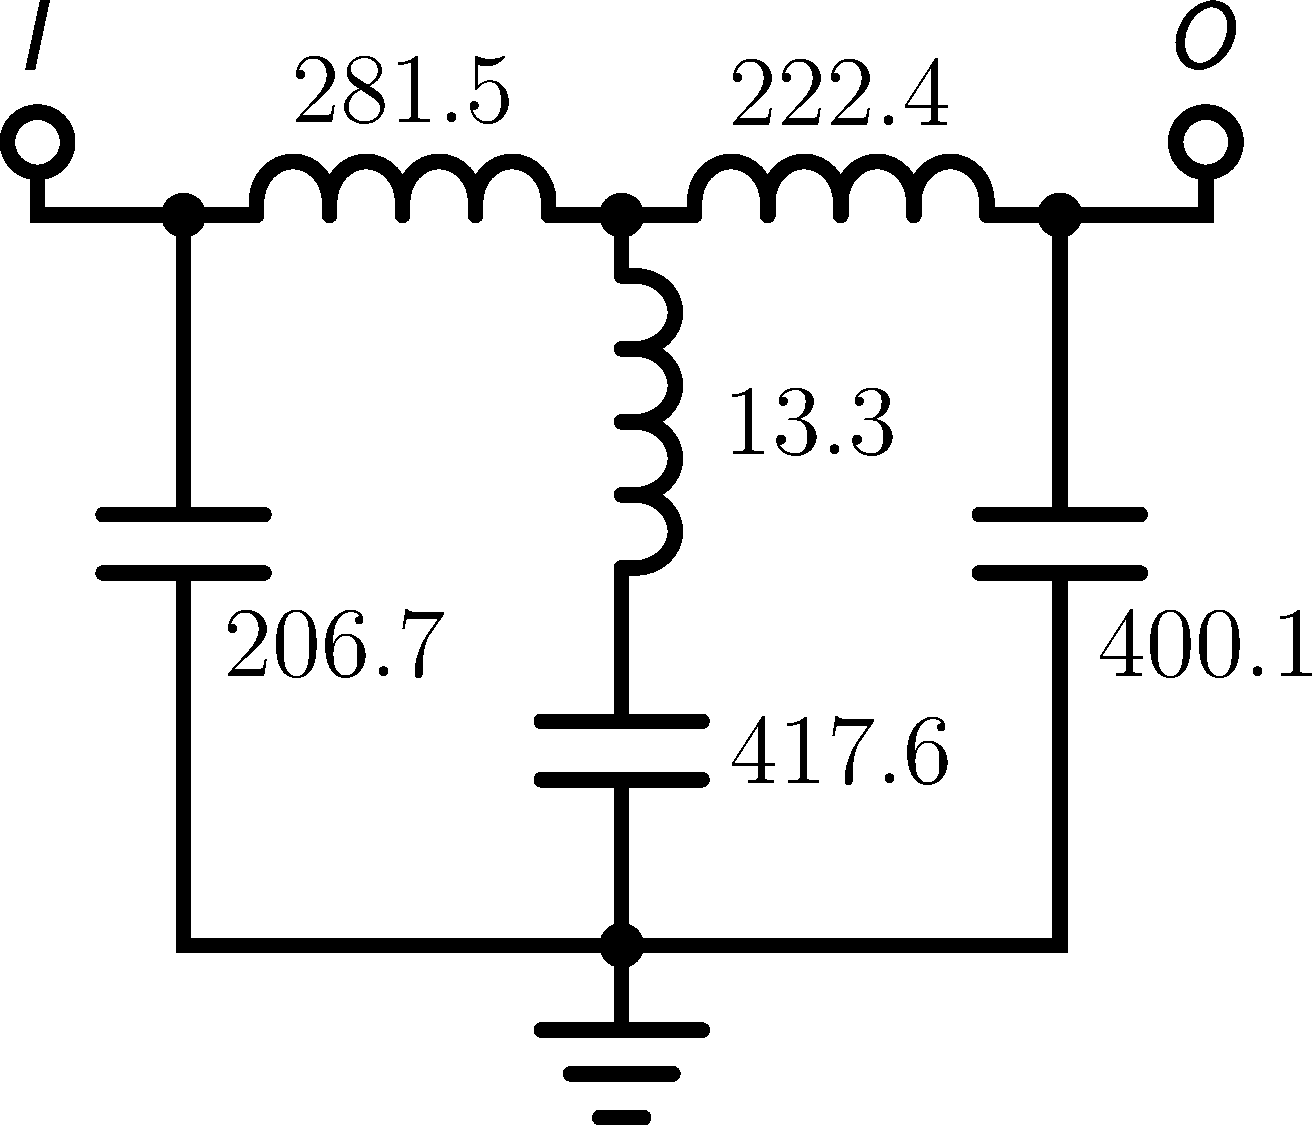
\includegraphics[scale = 0.14]{../app2/figures/(7)}
\caption{}
\end{subfigure}%
\begin{subfigure}[t]{0.25\textwidth}
\centering
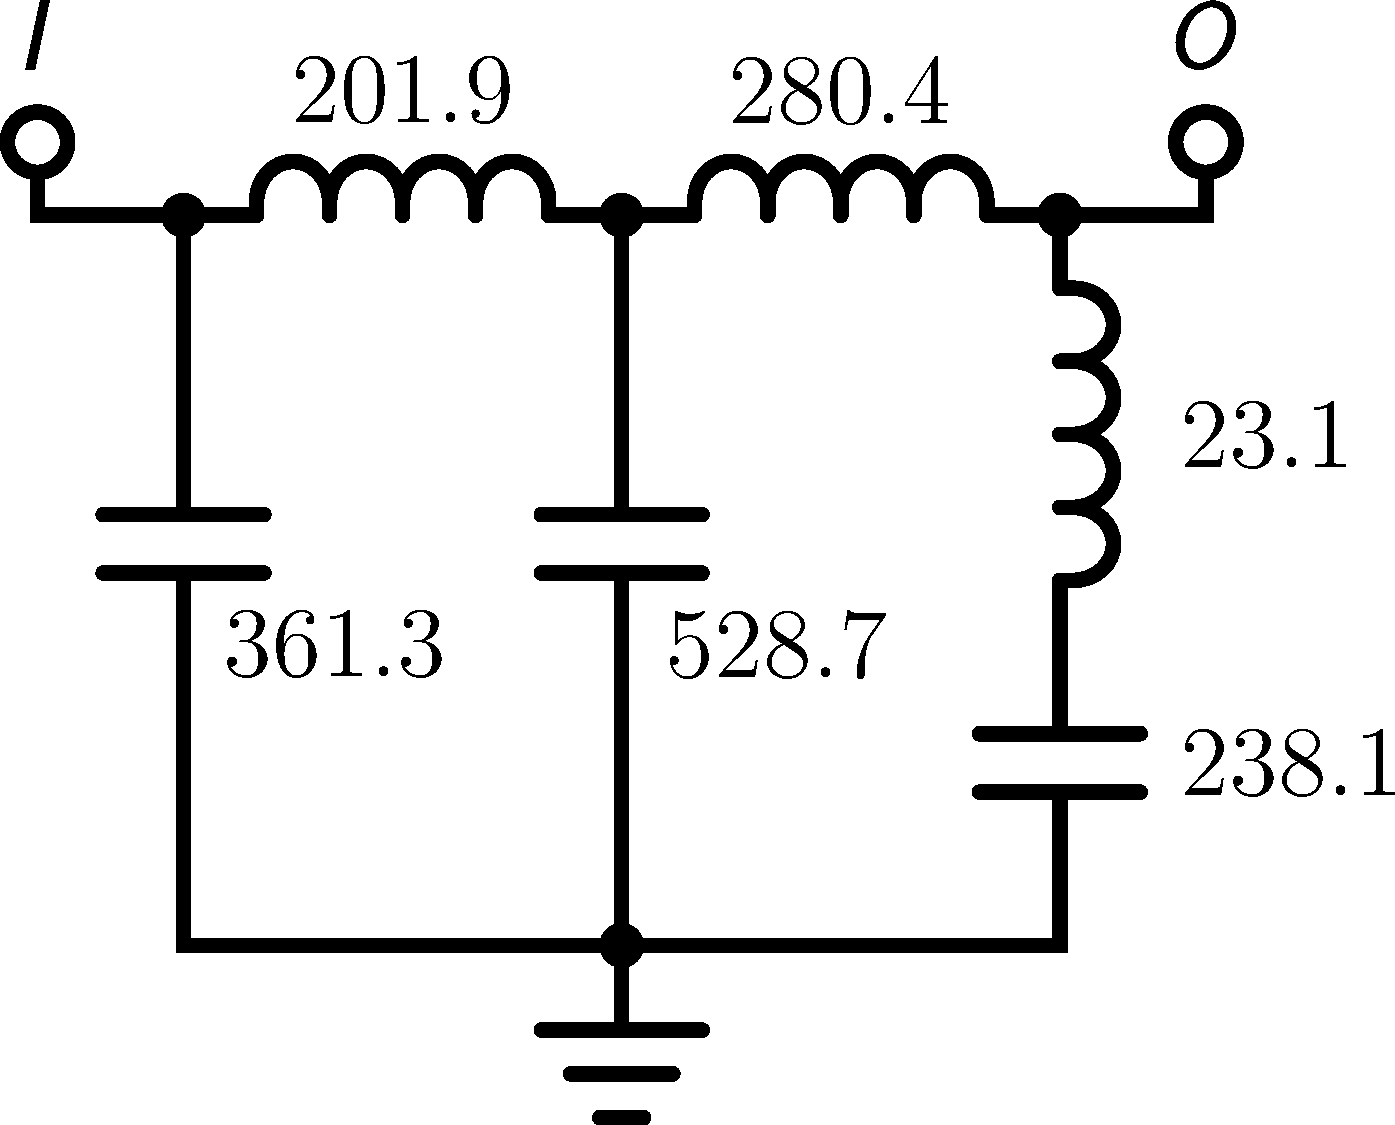
\includegraphics[scale = 0.14]{../ch6/figures/lpf3_circuit3}
\caption{}
\end{subfigure}%

\begin{subfigure}[t]{0.25\textwidth}
\centering
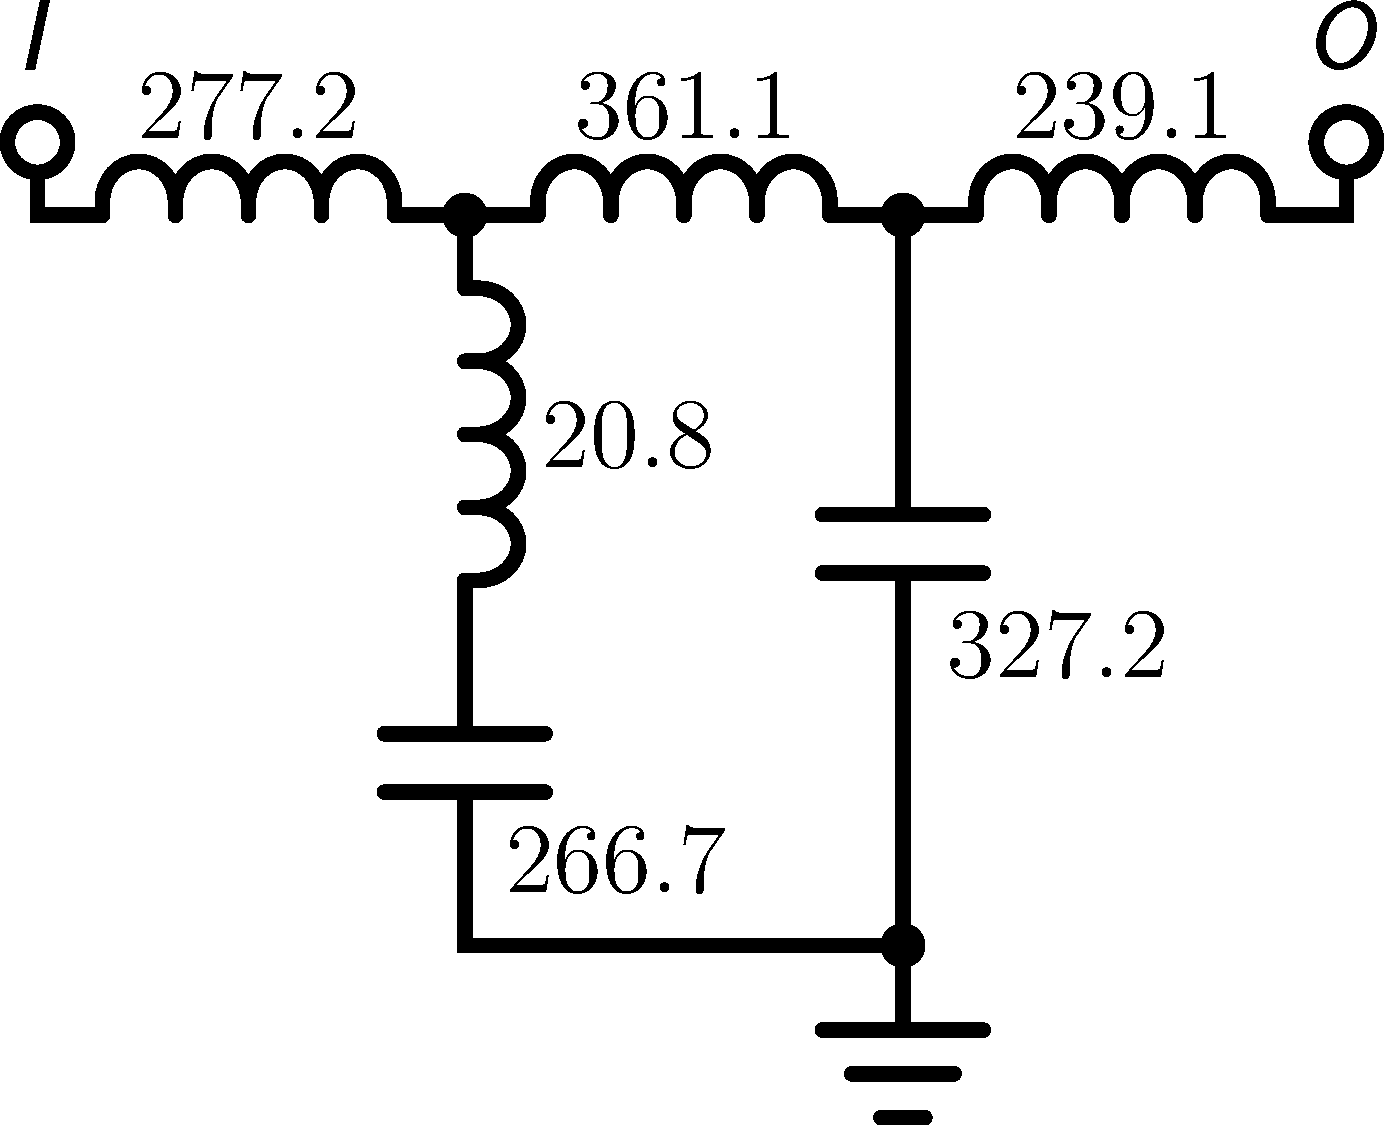
\includegraphics[scale = 0.14]{../app2/figures/(9)}
\caption{}
\end{subfigure}%
\begin{subfigure}[t]{0.25\textwidth}
\centering
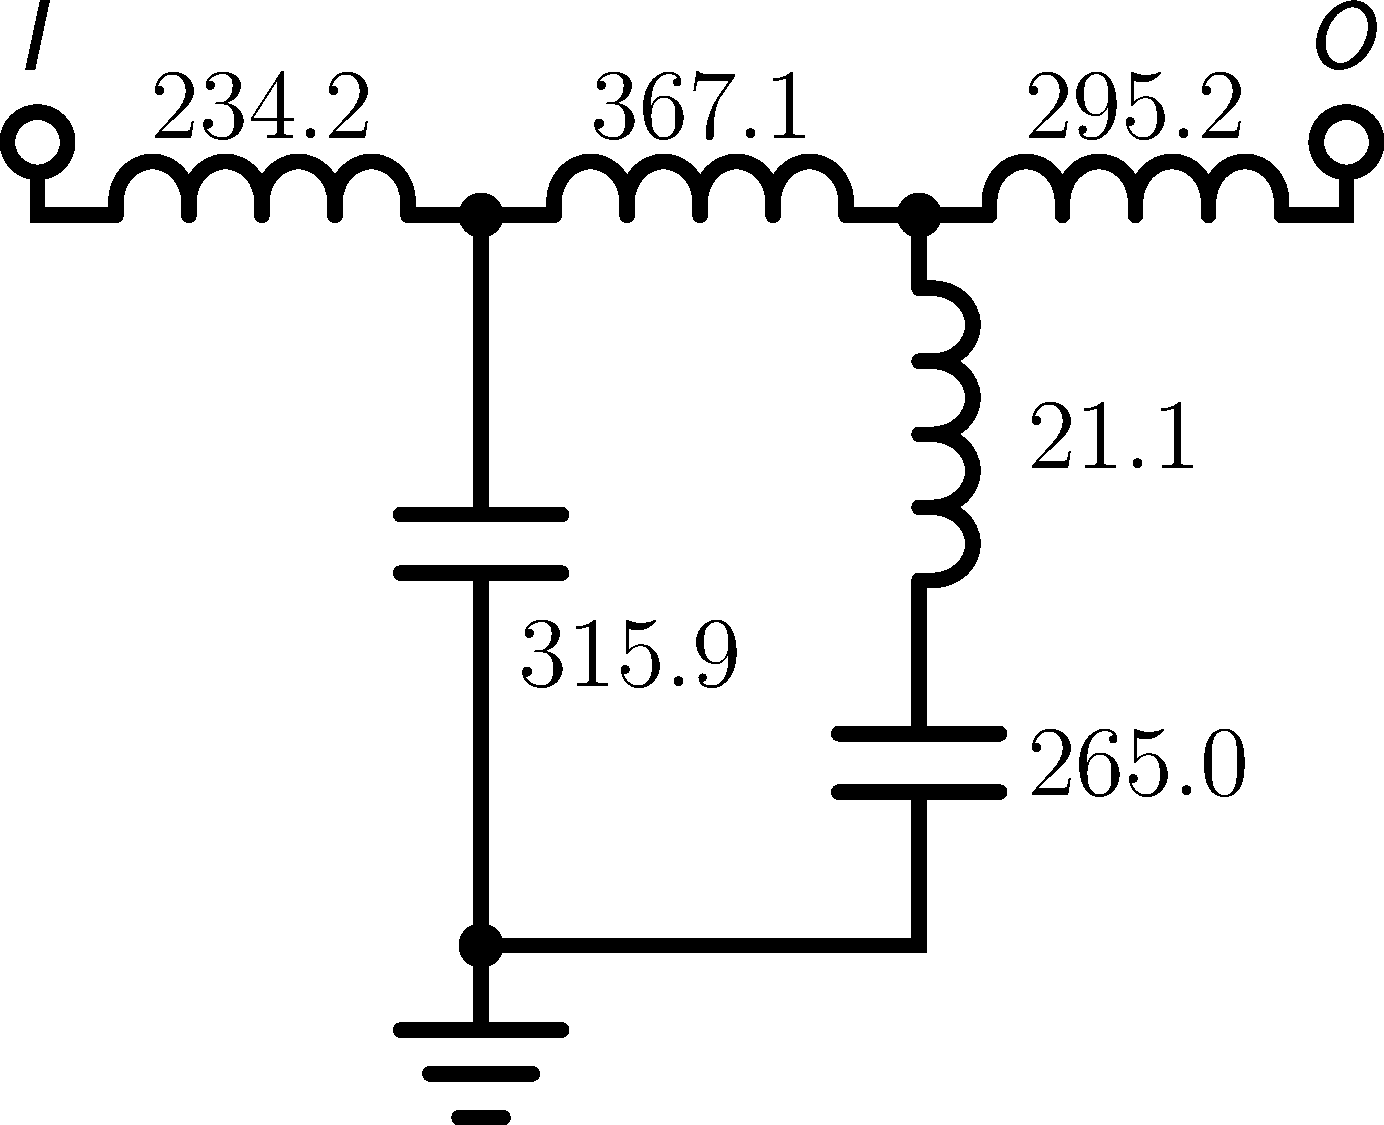
\includegraphics[scale = 0.14]{../app2/figures/(10)}
\caption{}
\end{subfigure}%

\caption[All ten minimum complexity topologies for \nameref{sec:ch6:lpf} task \#3.]{All ten minimum complexity topologies for \nameref{sec:ch6:lpf} task \#3 (units are mH and nF).\label{fig:app2:lpf3}}

\end{figure}

\begin{figure}[p]
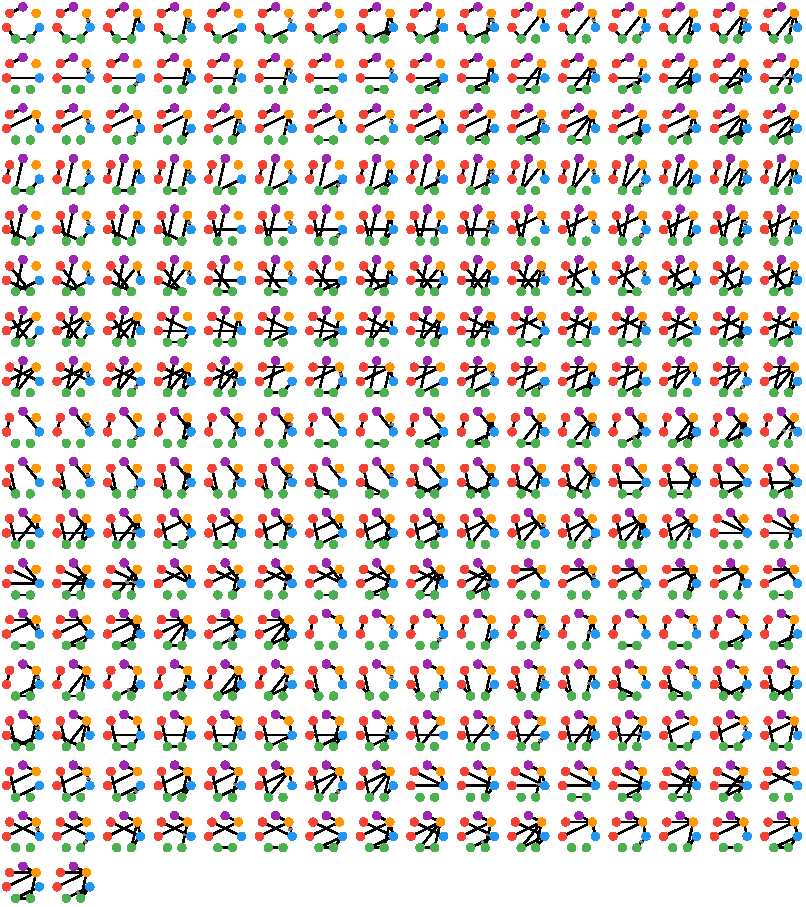
\includegraphics[width=\textwidth]{../app2/figures/ex2_allgraphs-reduced}
\caption{All 274 graphs in \nameref{sec:ch2:example2} with no additional \glsplural[noindex]{NSC} (gray hash indicates a multiedge).\label{fig:appB:example2}}
\end{figure}